\documentclass{article}
\usepackage[utf8]{inputenc}
\usepackage{amsmath}
\renewcommand{\thesubsection}{\thesection.\alph{subsection}}
\usepackage{titlesec}
\usepackage{amsmath}
\usepackage{mathtools}
\usepackage{amsthm}
\usepackage{amsfonts}
\usepackage{amssymb}
\usepackage{mathrsfs}
\usepackage{xcolor}

\titleformat{\subsection}[runin]
  {\normalfont\large\bfseries}{\thesubsection}{1em}{}
\titleformat{\subsubsection}[runin]
  {\normalfont\normalsize\bfseries}{\thesubsubsection}{1em}{}
\newcommand\tab[1][1cm]{\hspace*{#1}}


\title{Assignment 5 Relational Schema Design}
\author{Project Group 20:\\Jacob Dillie, Austin Lee, Ben Milas}
\date{Comp Sci 564 - Spring 2022}

\begin{document}

\maketitle
\section*{General Notes on Design}
Based on the constraints of the project, the key objectives in designing a good Entity-Relation model are speed and organization. Scalability was necessary for organizing the many-one relationships found in the Ebay JSON data.
\\\\
Many-one relationships include users (as sellers) to auctions, users (as bidders) to bids, items to classifications, and items to auctions. (Note that within the given data, each item was sold in exactly one auction, though it could be the case that an item is featured in multiple auctions.) Assuming the enumerated relations are possible, a minimum of five tables would be needed to accurately record all information from the JSON files.
\\\\
To minimize storage while maintaining organization, the group decided to use five tables and integer-valued primary keys only. After integer IDs associated with desired elements are found, a maximum of four searches would be needed to run any efficient query. When running on the CSL machines, constructing the databases and running the seven queries takes about six seconds total.
\section*{Relational Schema Definitions}
\textbf{ITEM} (\underline{itemID}::int, itemName::text)\\\\
\textbf{CLASSIFICATION} (\underline{classID}::int, itemID::int, categoryName::text)\\\\
\textbf{AUCTION} (\underline{auctionID}::int, itemID::int, sellerID::int, numBids::int, startPrice::double, \tab\tab currPrice::double, startTime::datetime, endTime::datetime)\\\\
\textbf{AUCTIONUSER} (\underline{userID}::int, userName::string, bidder::varchar(6), seller::varchar(6),\\ \tab\tab\tab rating::int, location::string, country::string)\\\\
\textbf{BID} (\underline{bidID}::int, auctionID::int bidderID::int, value::double, timeStmp::datetime)
\\
\pagebreak{}
\section*{\begin{center}Attributes\end{center}}
\begin{center}Auction\end{center}
\begin{center}
\begin{tabular}{|c|c|c|} 
 \hline
\textbf{Attribute} & \textbf{Key} & \textbf{Data Type}\\ [0.5ex] 
 \hline\hline
auctionID & PK & INT\\ \hline
itemID & FK & INT\\ \hline
sellerID & FK & INT\\ \hline
numBids & - & INT\\ \hline
startPrice & - & DOUBLE\\ \hline
currPrice & - & DOUBLE\\ \hline
startTime & - & DATETIME\\ \hline
endTime & - & DATETIME\\ \hline
\end{tabular}
\end{center}
\begin{center}AuctionUser\end{center}
\begin{center}
\begin{tabular}{|c|c|c|} 
 \hline
\textbf{Attribute} & \textbf{Key} & \textbf{Data Type}\\ [0.5ex] 
 \hline\hline
userID & PK & INT\\ \hline
userName & - & TEXT\\ \hline
bidder & - & VARCHAR(6)\\ \hline
seller & - & VARCHAR(6)\\ \hline
rating & - & INT\\ \hline
location & - & TEXT\\ \hline
country & - & TEXT\\ \hline
\end{tabular}
\end{center}
\begin{center}Bid\end{center}
\begin{center}
\begin{tabular}{|c|c|c|} 
 \hline
\textbf{Attribute} & \textbf{Key} & \textbf{Data Type}\\ [0.5ex] 
 \hline\hline
bidID & PK & INT\\ \hline
auctionID & FK & INT\\ \hline
bidderID & FK & INT\\ \hline
value & - & DOUBLE\\ \hline
timeStmp & - & DATETIME\\ \hline
\end{tabular}
\end{center}
\begin{center}Classification\end{center}
\begin{center}
\begin{tabular}{|c|c|c|} 
 \hline
\textbf{Attribute} & \textbf{Key} & \textbf{Data Type}\\ [0.5ex] 
 \hline\hline
classID & PK & INT \\ \hline
itemID & FK & INT \\ \hline
categoryName & - & TEXT \\ \hline
\end{tabular}
\end{center}
\begin{center}Item\end{center}
\begin{center}
\begin{tabular}{|c|c|c|} 
 \hline
\textbf{Attribute} & \textbf{Key} & \textbf{Data Type}\\ [0.5ex] 
 \hline\hline
itemID & PK & INT\\ \hline
itemName & - & TEXT\\ \hline
\end{tabular}
\end{center}
\pagebreak{}
\section*{\begin{center}Diagram\end{center}}
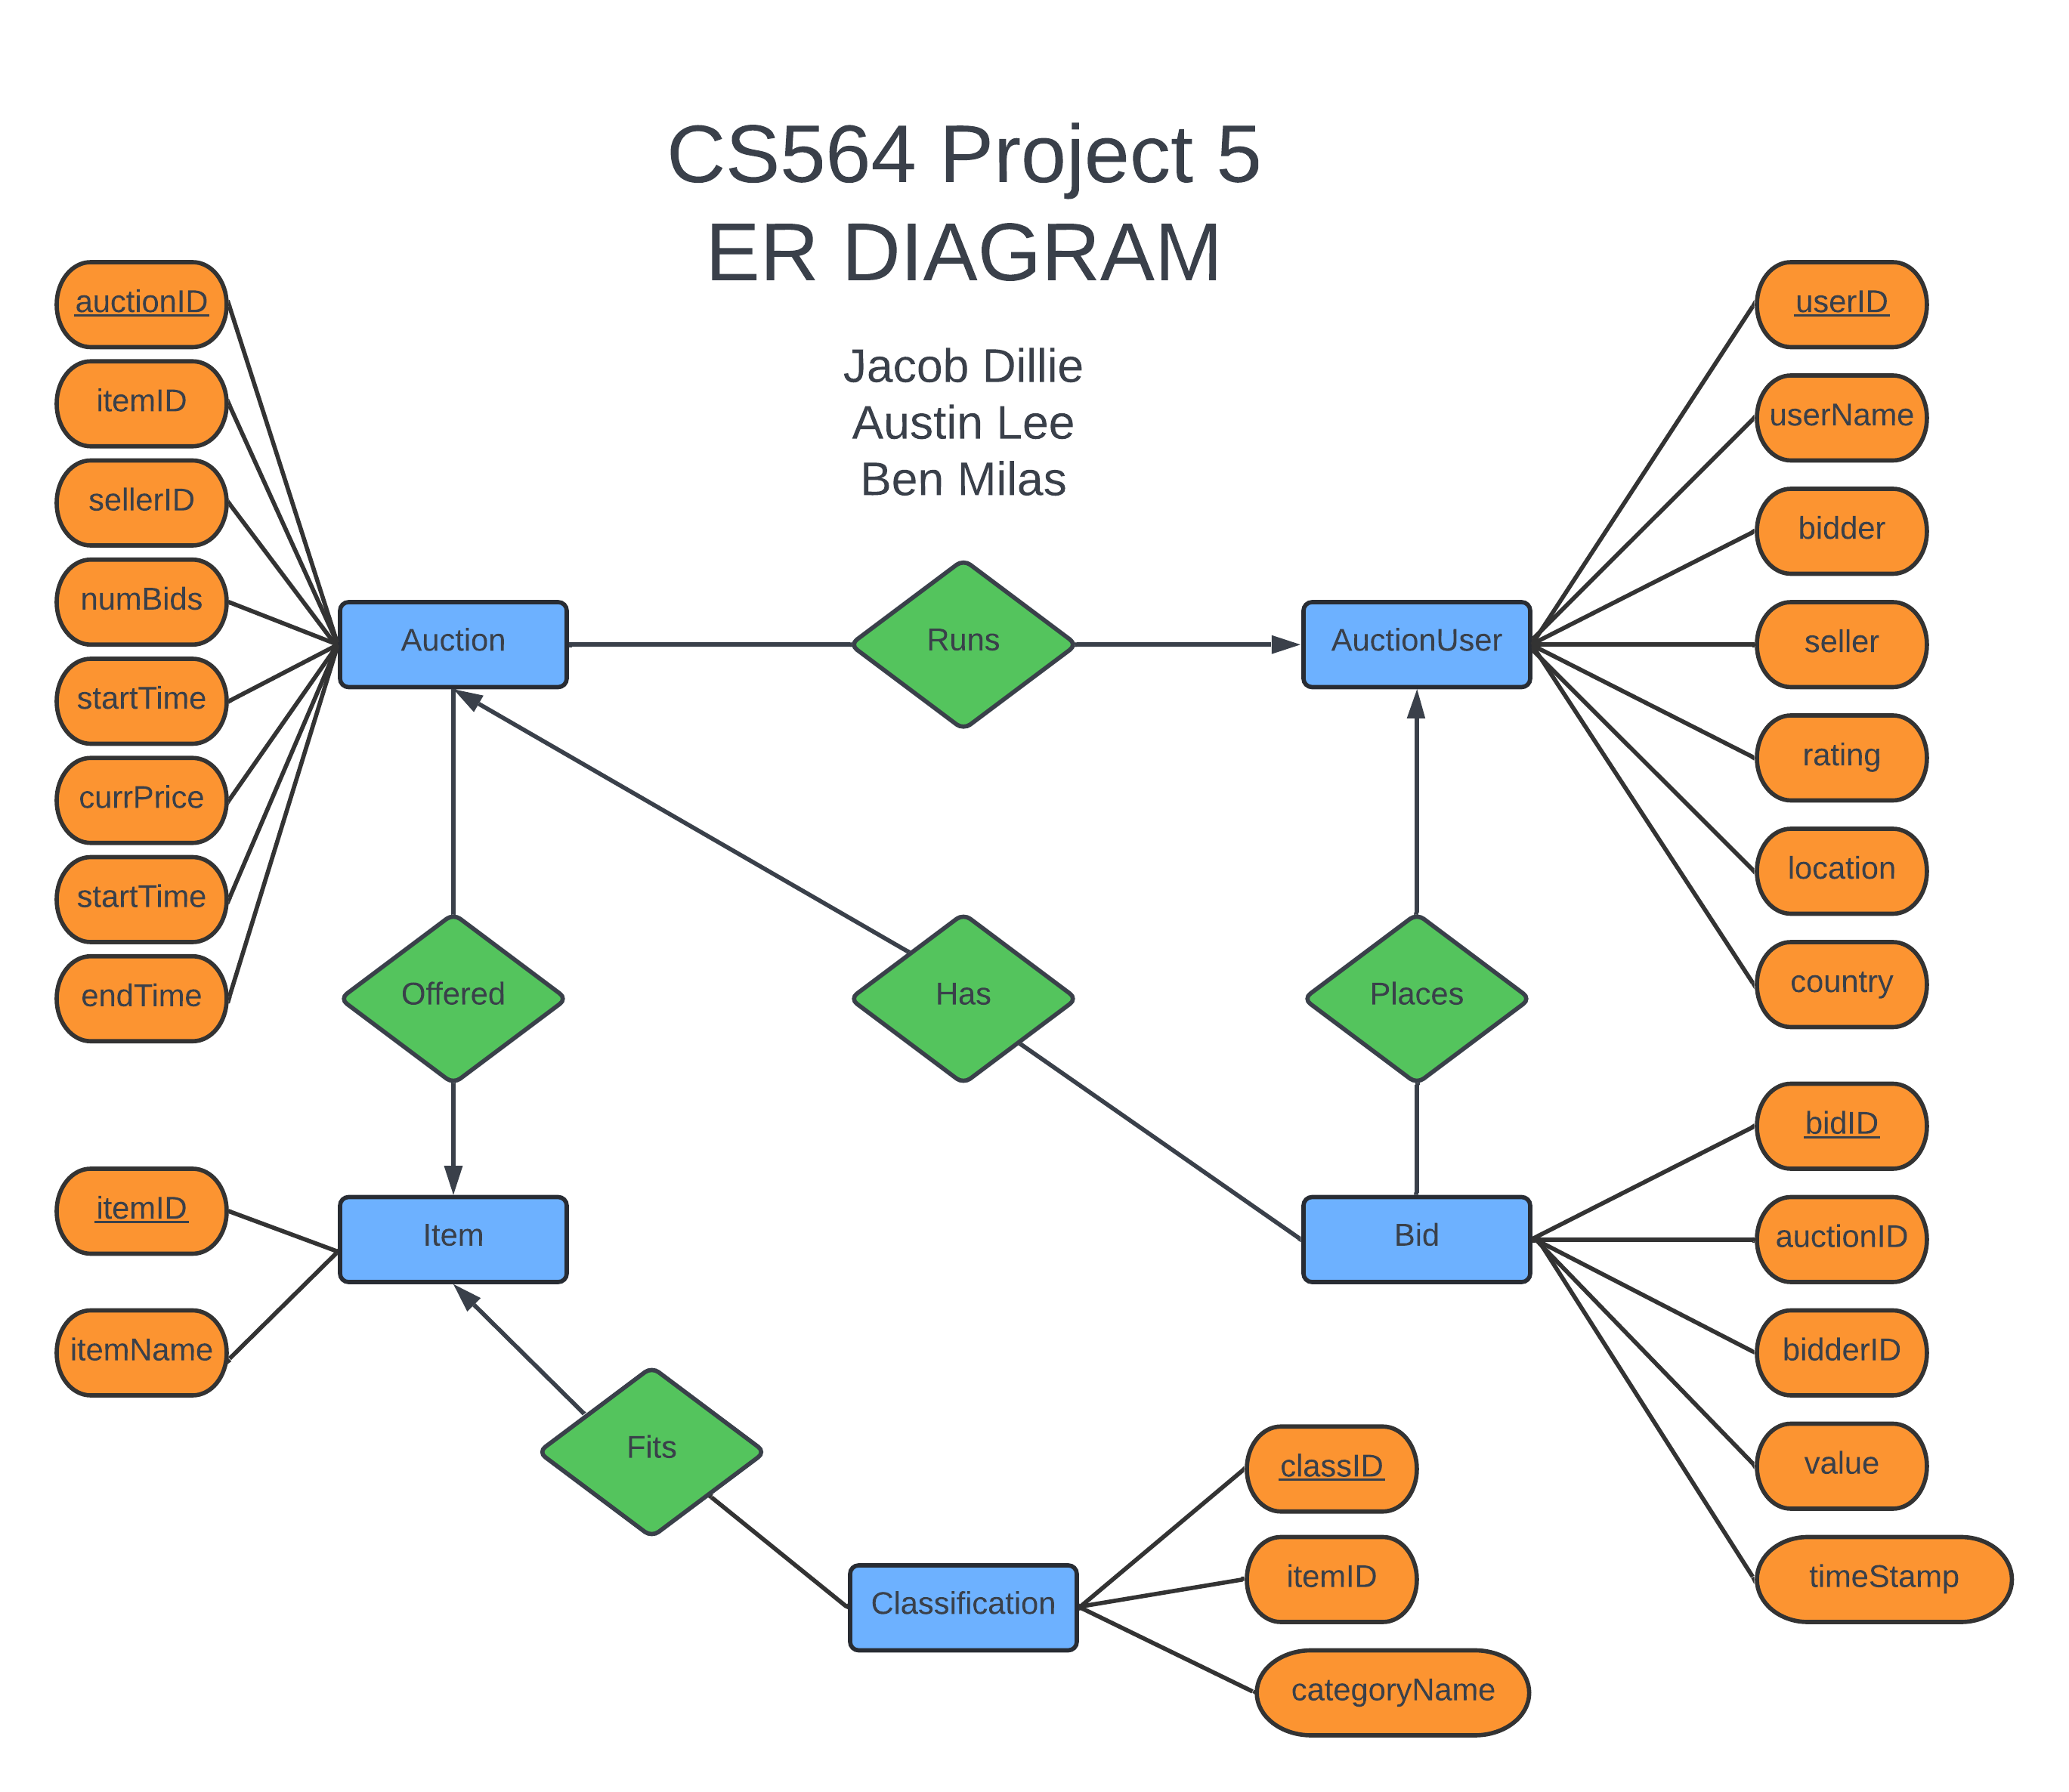
\includegraphics[scale=0.55]{erDiagram.png}
\end{document}
